\documentclass[border=10pt]{standalone}
\usepackage[svgnames]{xcolor}
\usepackage{amsmath}
\usepackage{pgfplots}
\pgfplotsset{compat=newest}
\usepackage[sfdefault]{FiraSans}
\usepackage{FiraMono}
\renewcommand*\familydefault{\sfdefault}
\begin{document}
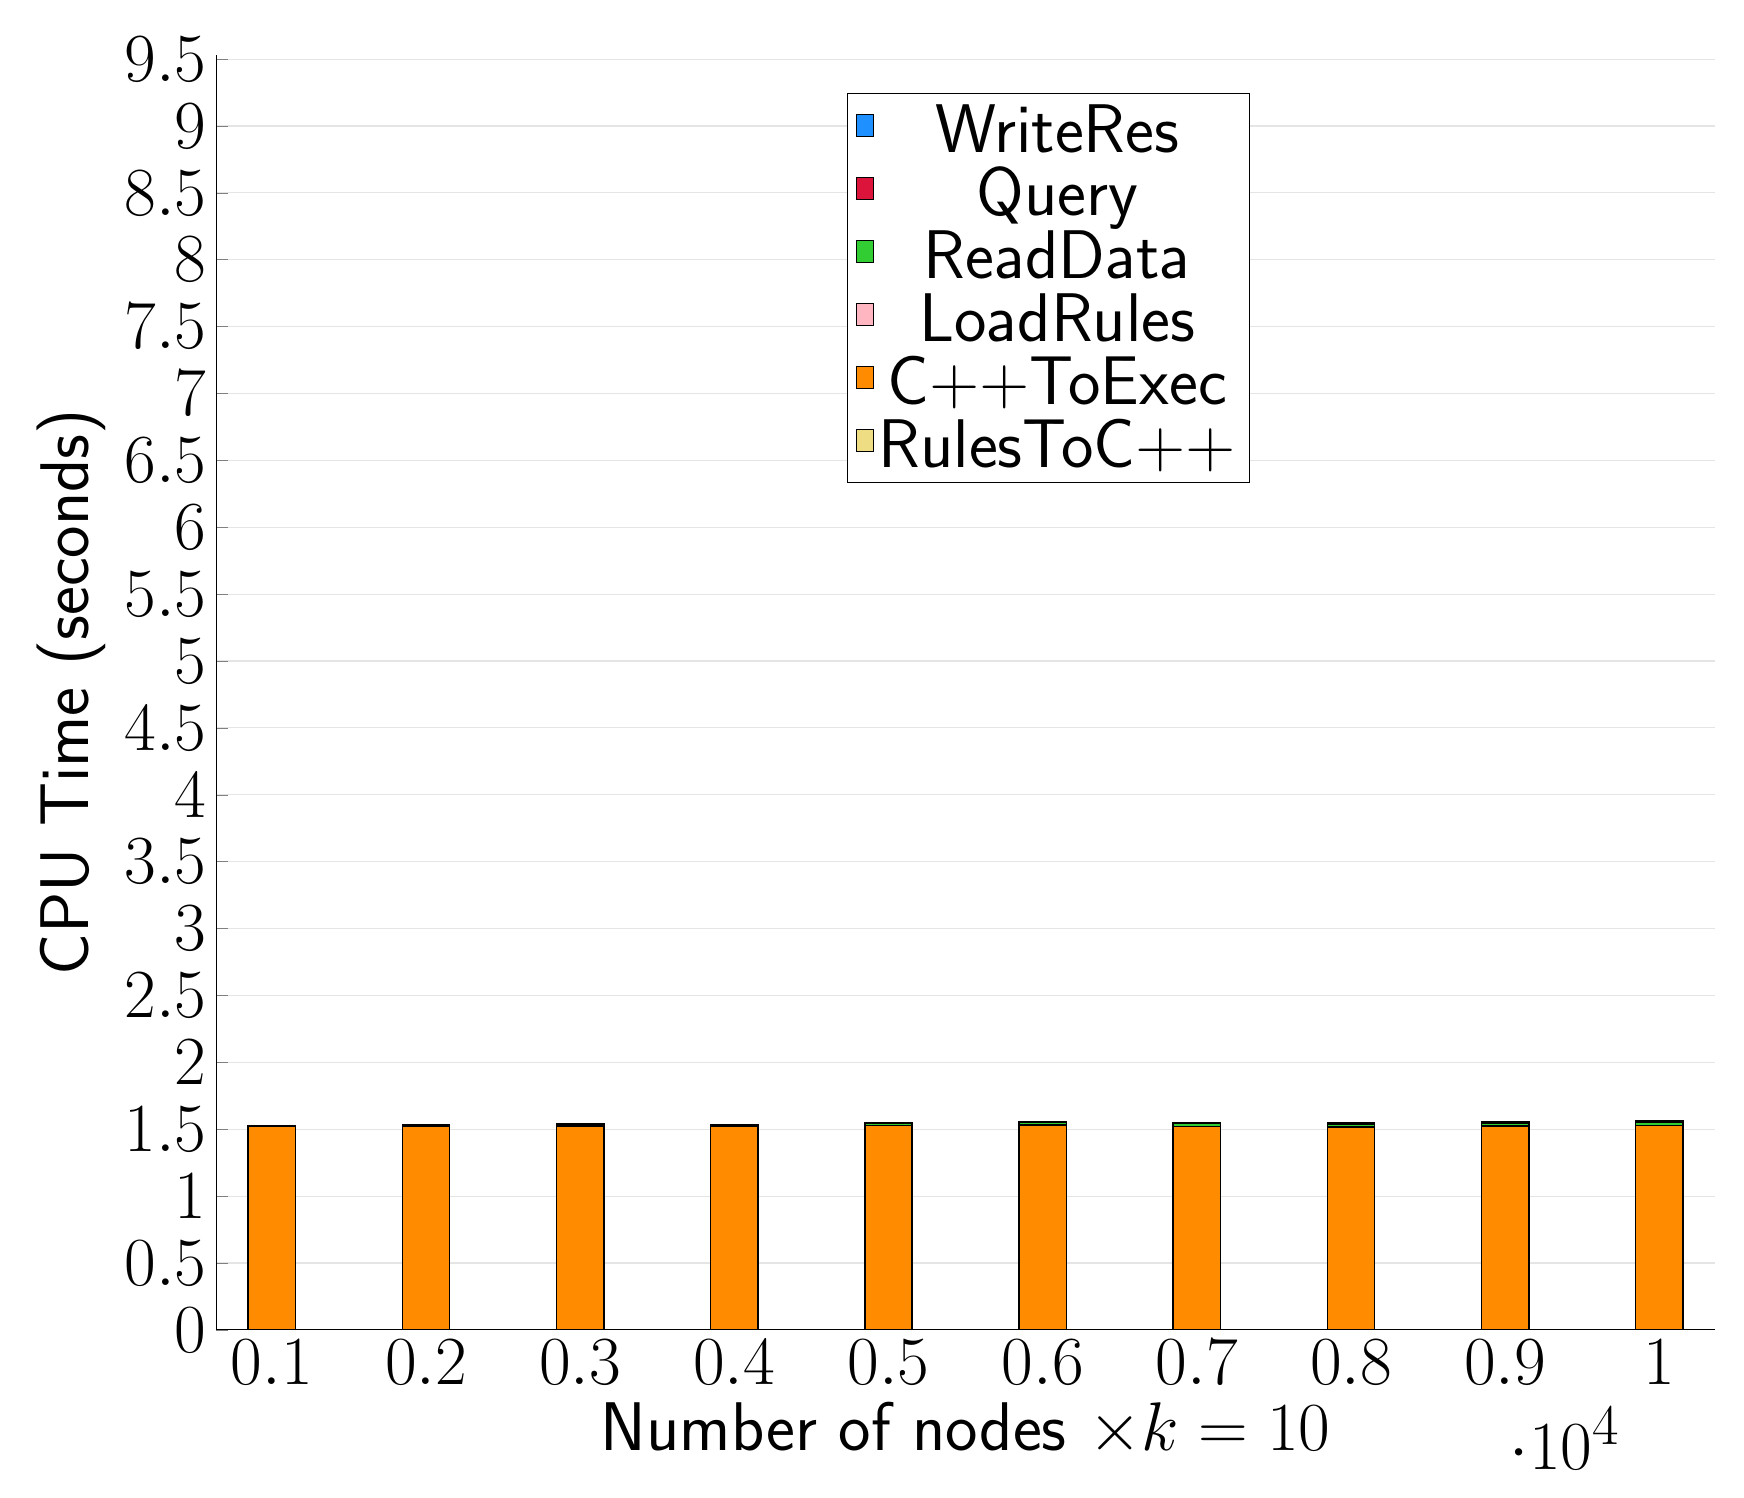
\begin{tikzpicture}
\begin{axis}[
   ybar stacked,
   width=1.7\textwidth,
   bar width=0.6cm,
   ymajorgrids, tick align=inside,
   major grid style={draw=gray!20},
   xtick=data,
   ymin=0, ymax=9.534,
   axis x line*=bottom,
   axis y line*=left,
   enlarge x limits=0.04,
   legend style={
       at={(0.69, 0.97)},
       anchor=north east,
       legend columns=1,
       font=\Huge,
   },
   ylabel={CPU Time (seconds)},
   xlabel={Number of nodes $\times k=10$},
   label style={font=\Huge},
   tick label style={font=\Huge},
]
\addlegendimage{fill=DodgerBlue, draw=black, line width=0.2pt}
\addlegendentry{WriteRes}
\addlegendimage{fill=Crimson, draw=black, line width=0.2pt}
\addlegendentry{Query}
\addlegendimage{fill=LimeGreen, draw=black, line width=0.2pt}
\addlegendentry{ReadData}
\addlegendimage{fill=LightPink, draw=black, line width=0.2pt}
\addlegendentry{LoadRules}
\addlegendimage{fill=DarkOrange, draw=black, line width=0.2pt}
\addlegendentry{C++ToExec}
\addlegendimage{fill=LightGoldenrod, draw=black, line width=0.2pt}
\addlegendentry{RulesToC++}
\addplot +[fill=LightGoldenrod, draw=black, line width=0.55pt] coordinates {
(1000, 0.0)
(2000, 0.0)
(3000, 0.0)
(4000, 0.0020000000000000005)
(5000, 0.0)
(6000, 0.0)
(7000, 0.0)
(8000, 0.0)
(9000, 0.0020000000000000005)
(10000, 0.004000000000000001)
};
\addplot +[fill=DarkOrange, draw=black, line width=0.55pt] coordinates {
(1000, 1.52)
(2000, 1.5260000000000002)
(3000, 1.526)
(4000, 1.518)
(5000, 1.528)
(6000, 1.532)
(7000, 1.5219999999999998)
(8000, 1.518)
(9000, 1.524)
(10000, 1.524)
};
\addplot +[fill=LightPink, draw=black, line width=0.55pt] coordinates {
(1000, 0.0001536)
(2000, 0.0001604)
(3000, 0.00015080000000000003)
(4000, 0.0001068)
(5000, 0.0001544)
(6000, 0.000142)
(7000, 0.0001536)
(8000, 0.0001352)
(9000, 0.0001298)
(10000, 0.00015140000000000002)
};
\addplot +[fill=LimeGreen, draw=black, line width=0.55pt] coordinates {
(1000, 0.004174)
(2000, 0.007274600000000001)
(3000, 0.0099366)
(4000, 0.010070800000000001)
(5000, 0.0144046)
(6000, 0.017011599999999998)
(7000, 0.0196324)
(8000, 0.0207322)
(9000, 0.022515)
(10000, 0.023981399999999996)
};
\addplot +[fill=Crimson, draw=black, line width=0.55pt] coordinates {
(1000, 0.0016581999999999999)
(2000, 0.0030346000000000006)
(3000, 0.0033034)
(4000, 0.0049546)
(5000, 0.0063923999999999995)
(6000, 0.0071556)
(7000, 0.008411199999999999)
(8000, 0.0090916)
(9000, 0.008910999999999999)
(10000, 0.010271800000000001)
};
\addplot +[fill=DodgerBlue, draw=black, line width=0.55pt] coordinates {
(1000, 0.0003872)
(2000, 0.000293)
(3000, 0.00022620000000000002)
(4000, 0.00024219999999999998)
(5000, 0.00026480000000000004)
(6000, 0.0002434)
(7000, 0.0002678)
(8000, 0.0002582)
(9000, 0.00022720000000000002)
(10000, 0.000256)
};
\end{axis}
\end{tikzpicture}

\end{document}
